\documentclass[conference]{IEEEtran}
\IEEEoverridecommandlockouts
% The preceding line is only needed to identify funding in the first footnote. If that is unneeded, please comment it out.
\usepackage{cite}
\usepackage{amsmath,amssymb,amsfonts}
\usepackage{algorithmic}
\usepackage{graphicx}
\usepackage{textcomp}
\usepackage{xcolor}
\usepackage{float}

\def\BibTeX{{\rm B\kern-.05em{\sc i\kern-.025em b}\kern-.08em
    T\kern-.1667em\lower.7ex\hbox{E}\kern-.125emX}}
\begin{document}

\title{Smart Fridge System: Intelligent Food Management and Health Integration\\
{\footnotesize \textsuperscript{}}
\thanks{}
}

\author{\IEEEauthorblockN{1\textsuperscript{st} Axel Lundin}
\IEEEauthorblockA{\textit{Acad. of Information Technology} \\
\textit{College of Halmstad}\\
Halmstad, Sweden \\
axelun22@student.hh.se}
\and
\IEEEauthorblockN{2\textsuperscript{nd} Aleksander Janokovic}
\IEEEauthorblockA{\textit{Acad. of Information Technology} \\
\textit{College of Halmstad}\\
Halmstad, Sweden \\
alejan22@student.hh.se}
\and
\IEEEauthorblockN{3\textsuperscript{rd} Mohammed ISMAILI}
\IEEEauthorblockA{\textit{Computer Science} \\
\textit{Al Akhawayn University}\\
Ifrane, Morocco \\
Mo.Ismaili@aui.ma}
\and
\IEEEauthorblockN{4\textsuperscript{th} Hyunsuk Lee}
\IEEEauthorblockA{\textit{Information Systems} \\
\textit{Hanyang University}\\
Seoul, South Korea \\
leehyunsuk2000@gmail.com}
}

\maketitle

\begin{abstract}
The app integrates with a smart refrigerator connected via wifi and synced with a fitness app. Equipped with cameras and an internal scale, the fridge helps users automatically track the nutrition values of the food they consume throughout the day. By leveraging real-time data from both the food recognition system and weight measurements, the app provides an accurate calculation of daily nutritional intake.

\end{abstract}

\section{Introduction}
\subsection{Motivation}
In an era where both health management and sustainability are increasingly critical, consumers are searching for solutions that can seamlessly integrate into their daily lives to help them achieve these goals. However, despite the proliferation of smart technologies in the home, existing smart fridges fall short in offering the tools necessary for comprehensive food management and nutritional tracking. These limitations make it difficult for users to manage their food consumption, track their caloric intake accurately, or reduce food waste effectively.

Our Smart Fridge System is designed to address these gaps by introducing a unique feature that current smart fridges lack: caloric intake tracking based on food weight. By integrating weight sensors and a nutritional database, our system enables users to track the exact amount of food consumed and automatically calculate the associated calories and macronutrients. This offers a precise and real-time method for managing daily food intake, which is especially valuable for users focused on personal health goals such as weight loss, maintenance, or muscle gain.

In addition to its nutritional tracking capabilities, our system is designed to simplify the process of meal planning. Through a user-friendly interface, the Smart Fridge can provide personalized meal recommendations based on the ingredients already available in the fridge and tailored to the user’s dietary preferences (e.g., vegetarian, low-carb). This reduces the time and effort needed for meal preparation while promoting healthier food choices that align with the user’s nutritional objectives.

One of the key challenges our system addresses is food waste, a growing environmental concern. Many households struggle to keep track of the food they have, leading to unnecessary waste as items expire unnoticed. Our Smart Fridge tackles this issue by sending alerts when food is nearing its expiration date and suggesting ways to use these ingredients before they spoil. This not only helps users make the most of the food they have but also contributes to the global effort to reduce food waste, promoting a more sustainable lifestyle.

The system is also designed to offer real-time insights into a user’s nutritional intake, providing daily and weekly summaries of calorie consumption and macronutrient distribution. Users can set personalized nutritionalgoals and track their progress over time, receiving visual feedback through charts and progress indicators. These features make it easier for users to stay on top of their dietary goals without relying on manual tracking methods, which can often be tedious and imprecise.

Unlike more complex solutions that attempt to integrate multiple external devices, such as fitness trackers, our Smart Fridge keeps the focus on accurate calorie tracking through weight-based measurements and food inventory management. By prioritizing this core functionality, we ensure that the system is both practical and achievable within the project’s timeframe, offering a real-world solution to the everyday challenges of food management and health tracking.

In summary, the Smart Fridge System provides a comprehensive and innovative approach to managing food consumption and nutritional health. By offering real-time calorie tracking, meal planning assistance, and food inventory management, the system enables users to make informed decisions about their diet while minimizing food waste. This project not only aligns with the growing demand for smarter, more sustainable household technologies but also addresses the need for more precise tools to help individuals achieve their personal health and fitness goals.
\subsection{Problem Statement}

\subsubsection{Need for Comprehensive Food Management}
Users require an efficient solution for tracking their food inventory and nutritional intake. Current technologies do not provide the ability to automatically monitor food consumption or alert users about expiring items, resulting in significant food waste. A system that can intelligently track food items, manage expiration dates, and reduce waste is essential.\\

\subsubsection{Desire for Integration with Health Management}
Many individuals struggle to maintain a balanced diet and track their caloric intake due to the lack of integration between food management systems and health monitoring tools. Clients need a refrigerator that can synchronize with fitness apps and wearable devices, providing personalized meal recommendations based on their dietary goals and caloric burn.\\

\subsubsection{Demand for Real-Time Nutritional Insights}
Consumers often lack the tools to obtain real-time nutritional information about the food they consume. A system that can calculate calories and macronutrients based on actual food intake, using weight measurements and food recognition technology, is necessary for helping users meet their health goals.\\

\subsubsection{Simplification of Meal Planning}
Users find meal planning cumbersome and time-consuming, often leading to poor dietary choices. Clients require an intelligent appliance that can suggest meal ideas based on the ingredients available, dietary preferences, and fitness objectives, thus simplifying the meal preparation process.\\

\subsubsection{Accessibility of Food Inventory Data}
Consumers desire a user-friendly interface that allows them to access and manage their food inventory easily. An app that provides seamless updates on what is left in the refrigerator and calculates nutritional intake would enhance the user experience, making it easier for individuals to make informed food choices.\\

\subsubsection{Reduction of Food Waste}
As food waste is a significant global issue, users are increasingly seeking ways to minimize their environmental impact. A system that notifies them of expiring items, generates grocery lists, and encourages the consumption of available food before spoilage is critical in addressing this concern.\\

\subsubsection{Support for Personal Health Goals}
Clients are looking for a solution that not only tracks food but also aligns with their personal health and fitness goals, such as weight loss or muscle gain. Integrating food management with fitness tracking will enable users to achieve their nutritional objectives more effectively.\\


\section{Requirements}
\subsection{User Authentication}
\subsubsection{Log-in}
Users will be able to log in to the app using their registered credentials (email/username and password). The app will securely authenticate user details by checking them against stored credentials in the database.\\

\subsubsection{Username}
Each user will choose a unique username during the signup process. The username will be used to identify the user in the app, along with other personal details.
Sign-up\\
Users will create an account by providing details like email, username, and password. The app will validate the provided information (e.g., checking if the email is already in use) before saving the user’s profile in the database.\\

\subsubsection{Password recovery}
If users forget their password, they can recover it via a password recovery process. The app will send a password reset link or OTP (One Time Password) to the registered email, allowing the user to set a new password.\\

\subsubsection{User profile}
Once logged in, users can manage their profile, which includes personal details like name, age, weight, height, and fitness goals (e.g., weight loss, muscle gain). This information helps the app calculate personalized nutrition recommendations.
Users can also update their dietary preferences (e.g., vegetarian, keto) and other health details to further personalize meal recommendations.\\\\

\subsection{Food Recognition \& Measurement}
\subsubsection{Intergration with a scale to measure food weight}
The app will determine the weight before and after to give an amount of used object. Combined with the food recognition system to calculate calorie content.
When the user places food on the scale, the app will display the real-time weight and automatically update when the weight changes.\\

\subsubsection{Camera/photo recognition for indenifying food items}
The app will track the weight of each item in the user’s fridge or pantry. When the user takes food out of the fridge or puts it back, they will weigh the item before and after, allowing the app to track the difference in weight (how much of the item was consumed or added).\\
For example, if a user weighs a block of cheese before eating and then weighs it again afterward, the app will calculate the difference in weight and associate the corresponding calorie intake with the amount consumed.\\
This feature ensures more precise calorie tracking since it accounts for the exact amount of food consumed.\\\\

\subsection{Calorie \& Nutrition Tracking}
\subsubsection{Real-time calculation of calories based on food weight and type}
The app will calculate calories in real-time based on the weight of food items detected by the refrigerator’s internal scale and the type of food identified by the camera or manual input. The system will use a comprehensive food database to determine the calorie content of different types of food and their respective portion sizes. As food is added or removed from the refrigerator, the app will automatically adjust the calorie count based on changes in weight.\\
\subsubsection{Daily and weekly summaries of calorie intake and macro nutrients}
The app will generate daily and weekly summaries that display the user’s calorie intake, broken down into macronutrients: carbohydrates, proteins, and fats. These summaries will help users review their eating habits over time and make informed adjustments to their diet. The data will automatically update as new food is added or consumed.\\

\subsubsection{Allow users to set calorie and macro nutrient goals (e.g.,
for weight loss, maintenance, or gain)}
Users can set personalized goals for daily calorie intake and macronutrient distribution (e.g., specific percentages for carbohydrates, proteins, and fats). The app will allow users to choose preset goals (e.g., for weight loss, maintenance, or muscle gain) or create custom targets based on their fitness objectives and dietary preferences. The system will compare the user’s actual intake against their goals and provide feedback to help them stay on track.\\

\subsubsection{Graphical representation of progress toward goals}
The app will provide a graphical representation of the user’s progress toward their daily and weekly calorie and macronutrient goals. Color-coded charts will differentiate between macronutrients (e.g., fats, carbs, proteins), showing users how close they are to meeting their targets. Users will also be able to track trends over time, helping them adjust their eating habits based on their progress. Alerts and notifications will be provided if the user is falling behind or exceeding their calorie or macronutrient goals.


\subsection{Meal Recommendations}
Personalized meal suggestions based on user goals, dietary preferences, and daily progress. With personalized meal suggestions it allows the user to easily make meals depending on the fridge inventory that suits the users needs.\\\\
Option to filter recommendations (e.g., vegetarian, low-carb, high-protein), by providing an option to allow users to filter recipes it will make meal suggestions even more directed to the user

\subsection{User Goals \& Progress}
Setting weight goals and tracking progress over time, this allows users to set personalized weight goals and continuously monitor progress through food consumption data and weight changes\\
Monitoring nutritional goals (calories, protein, carbs, fats), Provides insights into daily intake of calories and macronutrients, helping users stay on track with nutritional objectives.\\
Integration with wearable devices for activity tracking and calorie burn estimates, Syncs with fitness wearables to incorporate activity data, offering real-time calorie burn insights for a comprehensive view of intake versus expenditure.

\subsection{Usability}
Intuitive design for easy food logging and tracking:\\
Make a user-friendly app for logging and tracking food that stores it in a database for the user to see its progress
Clear guidance for setting and achieving goals\\
The user should be able to set its goals such as weight.

\section{Development Environment}
\subsection{Choice of software development platform}
The initial goal of the project was to develop a mobile application for the smart fridge system, aiming to provide users with a seamless, on-the-go interface for tracking food inventory and nutrition. A mobile app was chosen for its portability and accessibility, aligning with the modern preference for mobile-first solutions.
However, due to time constraints and the complexity of developing a fully functional mobile app within the project timeline, we opted to focus on creating a web application. This decision allowed us to deliver a working prototype that demonstrates the system's core functionalities while still reflecting the intended user experience.

\subsection{Programming Languages}
\begin{itemize}
    \item Python was the backbone for our system and machine learning workflows. It was chosen for its simplicity, versatility and its many different libraries. This made it an ideal choice for developing our smart fridge system. Libraries such as Flask, TensorFlow, Keras, OpenCV and Numpy all played a crucial role in our project development.
    \begin{itemize}
        \item Backend Development: Flask was used to develop the backend API and handle server-side logic. It was chosen due to its lightweight framework but also because of its simplicity and scalability.
        \item Image Processing: OpenCV, a python library used for handling video streams as well as image manipulation. These features were crucial for the core function of our project.
        \item Machine Learning: TensorFlow is a machine learning framework which enabled us to implement our own Convolutional Neural Network (CNN) for food recognition. Keras also provided a user-friendly interface for building and testing the architecture.
        \item Numpy was utilized for its efficiency when preprocessing image data and managing arrays during machine learning workflows. Its speed and reliability also played a role in using the Numpy library.
    \end{itemize}
    \item JavaScript allowed interactivity to the web application which made it dynamic and responsive to user inputs. It also provided real-time updates and integrated the frontend with Cloud Firestore, allowing a seamless communication between the database and the user interface.
    \item HTML provided our structure for the web application by defining the layout and content hierarchy.
\end{itemize}
\subsection{Firebase and Firestore (NoSQL)}
Firestore, a NoSQL database provided by Firebase, played a critical role in data storage and real-time synchronization. Firestore also allows for scalability as the system grows and its ease of use when adding features such as authentication reduced the development complexity.
\begin{itemize}
    \item Reat-Time Synchronization, ensured that user data (e.g food inventory, nutrional tracking) was always up-to-date. For example when the user eats a food item the database is updated allowing the user to view changes immediately.
    \item Integration with Python SDKs, functions in Python were used to query Firestore for nutritional information and to save user-specific records, such as daily caloric intake and progress tracking.
    \item Data Consistency, Food inventory, user profiles, and nutritional data were stored in a structured format, ensuring consistency with the machine learning model’s outputs.
\end{itemize}

\subsection{Hardware and Software Resources}
\begin{itemize}
    \item Operating System: Windows 11, 64-bit
    \item Backend Framework: Flask 2.3.2
    \item Machine Learning: TensorFlow 2.14.0
    \item Image Processing: OpenCV 4.8.0
    \item Database: Google Cloud Firestore
    \item Frontend: HTML and JavaScript (including Firebase SDKs)
    \item Version Control: Git and GitHub for source code management and collaboration.
    \item Computer Specifications
    \begin{itemize}
        \item Processor: Intel Core i7, 11th Gen
        \item RAM: 16GB
        \item GPU: Intel Iris Xe Graphics
        \item Storage: 256GB SSD
    \end{itemize}
\end{itemize}

\subsection{Cost Estimation}
Our selected development setup is mainly budget-friendly:\newline
Development Software: No cost, utilizing windows and free tools like Python, OpenCV, and TensorFlow.
If additional storage and processing power are needed, we may consider using Amazon Web Services (AWS). This can provide scalability and security for real-time data processing but will vary in cost depending on usage.

\section{Specifications}
In this section, we outline the specific implementation details for the main features of the Smart Fridge System, including food recognition, nutritional tracking, meal recommendations, and user goal tracking. Each specification is designed to provide a comprehensive solution to user needs, as detailed below.
\subsection{Food Recognition and Measurement}
To accurately track food intake, our system employs a combination of image recognition and weight measurement:\newline
    1. Image Recognition:\newline
         Using OpenCV with a TensorFlow or PyTorch model, the system captures images of food items placed in the fridge. The image recognition model identifies the food item and categorizes it by type.\newline
         Implementation: A camera module within the fridge captures images, which are processed using OpenCV for initial image processing, such as resizing and normalization. The processed images are then input into a pre-trained machine learning model that classifies the food type with a specified confidence threshold.\newline
         Technical Details: The model is trained on a dataset of common food items, ensuring accuracy for frequently consumed foods. Post-processing adjusts the output to filter and confirm results.\newline
    2. Weight Measurement:\newline
        The fridge uses an internal scale to measure the weight of food items. Before and after each use, the weight is recorded to determine consumption.\newline
        Implementation: Weight data is processed through the application to calculate consumed portions. A food item’s initial and final weights are compared, and the difference determines the amount consumed.
        Technical Details: Weight measurements are stored in the database with timestamps, and a smoothing algorithm accounts for minor fluctuations to ensure accuracy.\newline
\subsection{Nutritional Tracking}
To provide accurate nutritional data and enable health tracking:\newline
    1. Caloric and Macronutrient Calculation:\newline
         Each identified food item is cross-referenced with a dietary database (e.g., USDA Food Composition Database) to retrieve nutritional values.
         Implementation: Once a food item is identified and its weight calculated, the system accesses the dietary database for calorie, protein, fat, and carbohydrate values. Nutritional values are then stored in a user’s daily log.\newline
         Technical Details: Calculations are adjusted for portion size and weight, and data is updated in real time to reflect the user’s cumulative daily intake.\newline
    2. User Goals and Progress Tracking:\newline
         Users can set goals for daily calorie intake and specific macronutrient distribution, such as high protein or low carbohydrate intake.\newline
         Implementation: The system tracks nutritional intake against these goals, providing alerts and progress reports. Data visualization tools display daily and weekly summaries, highlighting trends and goal adherence.\newline
         Technical Details: Data visualizations are created using libraries such as Matplotlib or Plotly, allowing users to easily track their progress toward nutritional targets.\newline
\subsection{Personalized Meal Recommendations}
The system recommends meals based on available ingredients and user-defined dietary preferences:\newline
    1. Recipe Matching:\newline
         Using the identified inventory, the system suggests recipes aligned with user goals and available ingredients.\newline
         Implementation: An algorithm matches the food inventory against a preloaded recipe database, filtering results by user dietary preferences (e.g., vegetarian, low-carb).\newline
         Technical Details: Each recipe is tagged with dietary attributes, and an SQL query retrieves relevant options from the database based on user input.\newline
    2. Grocery List Generation:\newline
         The system generates a grocery list based on recipes chosen by the user and available inventory.\newline
         Implementation: When a recipe is selected, the system compares its ingredient list with the fridge’s inventory and adds any missing items to the grocery list.\newline
         Technical Details: Inventory is updated automatically as items are used, and the grocery list is stored in the database for easy access.
\subsection{Food Waste Reduction}
To help users minimize waste, the system monitors food expiration dates and usage:\newline
    1. Expiration Alerts:\newline
        The system tracks the expiry dates of stored items, alerting the user when items are close to expiration.\newline
        Implementation: Users input expiration dates upon adding items, and the system sends reminders as the date approaches.\newline
        Technical Details: A daily background process checks for items within the expiration threshold, triggering notifications when needed.
    2. Usage Suggestions for Expiring Items:\newline
        For items near expiration, the system suggests recipes to encourage usage before they spoil.\newline
        Implementation: When an item approaches expiration, the system searches for recipes that use the item and suggests them to the user.
        Technical Details: The algorithm prioritizes expiring items in the recipe search to minimize waste, drawing from the same recipe database.\newline

\section{Architecture Design and Implementation}
\subsection{Overall Architecture}

Our architecture consists of three main parts: the app frontend, backend servers, and the database.

1. **App Frontend**  
The frontend application provides an intuitive user interface for managing food inventory and tracking nutritional information. Users log in using Firebase Authentication, which retrieves their information and authentication keys for backend identification. The app displays real-time updates on food items and nutritional data, enabling users to interact with their smart fridge effectively.

2. **Backend Servers**  
   - **Main Server**: Acts as the central hub for data processing and storage. It handles user requests and manages interactions between the frontend and various backend services. User routines, preferences, and settings are stored here and retrieved upon user login via a RESTful API.
   
   - **AI Processing Server**: This server analyzes video feeds from cameras to recognize food items and monitor user interactions. It processes frames to detect presence and actions, determining what food items are available and how they can be used.
   
   - **Media Server**: A separate server runs software that connects to cameras, providing a static IP for both frontend and backend access. The RTMP protocol is used to stream video from the camera to the AI Processing server for analysis. The HLS protocol is employed for receiving video streams from the frontend.

3. **Database**  
   - **Firestore (NoSQL)**: Firestore plays a critical role in data storage and real-time synchronization. It ensures that user data (e.g., food inventory, nutritional tracking) is always up-to-date. Integration with Python SDKs allows querying Firestore for nutritional information and saving user-specific records.

4. **User Interaction and Notifications**  
When a user logs in, Firebase Authentication ensures secure access to personalized data. The system sends notifications about food expiration dates and suggests recipes based on available ingredients. If a user’s routine is triggered by detected actions (e.g., logging food consumption), relevant data is sent to the frontend using Firebase Cloud Messaging (FCM), prompting the app to execute associated routines.

This architecture provides a robust framework for managing food inventory and nutrition tracking while ensuring seamless interaction between users and their smart fridge environment.
\subsection{Directory Organization}
The directory structure for the Smart Fridge project ensures a clear and modular organization to streamline development, testing, and deployment. Below is the structure and explanation:
\clearpage
\begin{table}[H]
    \centering
    \caption{Directory Organization}
    \label{tab:directory_organization}
    \resizebox{\textwidth}{!}{ % Automatically adjusts to the text width
    \begin{tabular}{|l|p{3cm}|p{7cm}|}
        \hline
        \textbf{Directory/File} & \textbf{Type} & \textbf{Description} \\\hline
        \texttt{/Data} & 
        \raggedright \texttt{calorie\_data.json}, \newline \texttt{databaseInfo.py}, \newline \texttt{fruit\_classifier\_model.h5}, \newline \texttt{label\_dict.json} & 
        Data module containing dataset files, machine learning models, and helper files for data preprocessing. \\ \hline
        \texttt{/Data/images} & \texttt{.gitkeep} & Folder for storing \newline image data used \newline during training or \newline prediction processes. \\ \hline
        \texttt{/website} & \texttt{\_\_init\_\_.py}, \texttt{firebase.py}, \texttt{models.py}, \texttt{views.py}, \texttt{calculateIndv.py} & Core backend \newline modules including \newline Firebase integration, \newline routes, and \newline calculations. \\ \hline
        \texttt{/website/templates} & \texttt{base.html}, \texttt{modifyUser.html}, \texttt{userReg.html}, \texttt{createUser.html} & Frontend templates \newline defining the user \newline interface for various \newline parts of the \newline application. \\ \hline
        \texttt{/website/static/js} & \texttt{auth.js}, \texttt{modifyUser.js}, \texttt{createUser.js}, \texttt{prediction.js} & Client-side \newline JavaScript files \newline handling dynamic \newline functionality in the \newline frontend, like user \newline authentication. \\ \hline
        \texttt{/notebooks} & \texttt{.gitkeep} & Placeholder for \newline analysis or \newline exploratory data \newline processing \newline notebooks (optional). \\ \hline
        Root & \texttt{requirements.txt}, \texttt{README.md} & Root-level files for \newline server configurations \newline and project \newline information. \\ \hline
    \end{tabular}
    }
\end{table}
\clearpage
\subsection{Core Modules and Components}
\subsubsection{views.py (Routing and Request Handling)}  
\begin{itemize}
    \item Purpose: Acts as the backbone of the application by linking user requests to the appropriate backend logic and frontend templates.\newline
    \item Key Functionalities: \newline
           Routing: Defines endpoints for user actions like login, registration, modifying user data, and predictions.\newline
           File Handling: Processes user-uploaded files (images/videos) for prediction tasks.\newline
           Data Fetching: Retrieves user-specific nutritional data and updates it dynamically based on predictions.\newline
    \item Notable Endpoints:\newline
            /predict: Handles file uploads, processes predictions, and updates Firebase with nutritional information.\newline
            /fetchdate: Fetches user-specific data for selected dates, allowing users to track progress.\newline
            /createUser: Collects and calculates user-specific goals (calorie, protein, fat, and carbohydrate targets) and stores them in the database.\newline
    \item Graphical Representation: \newline
    \begin{figure}[H]
        \centering
        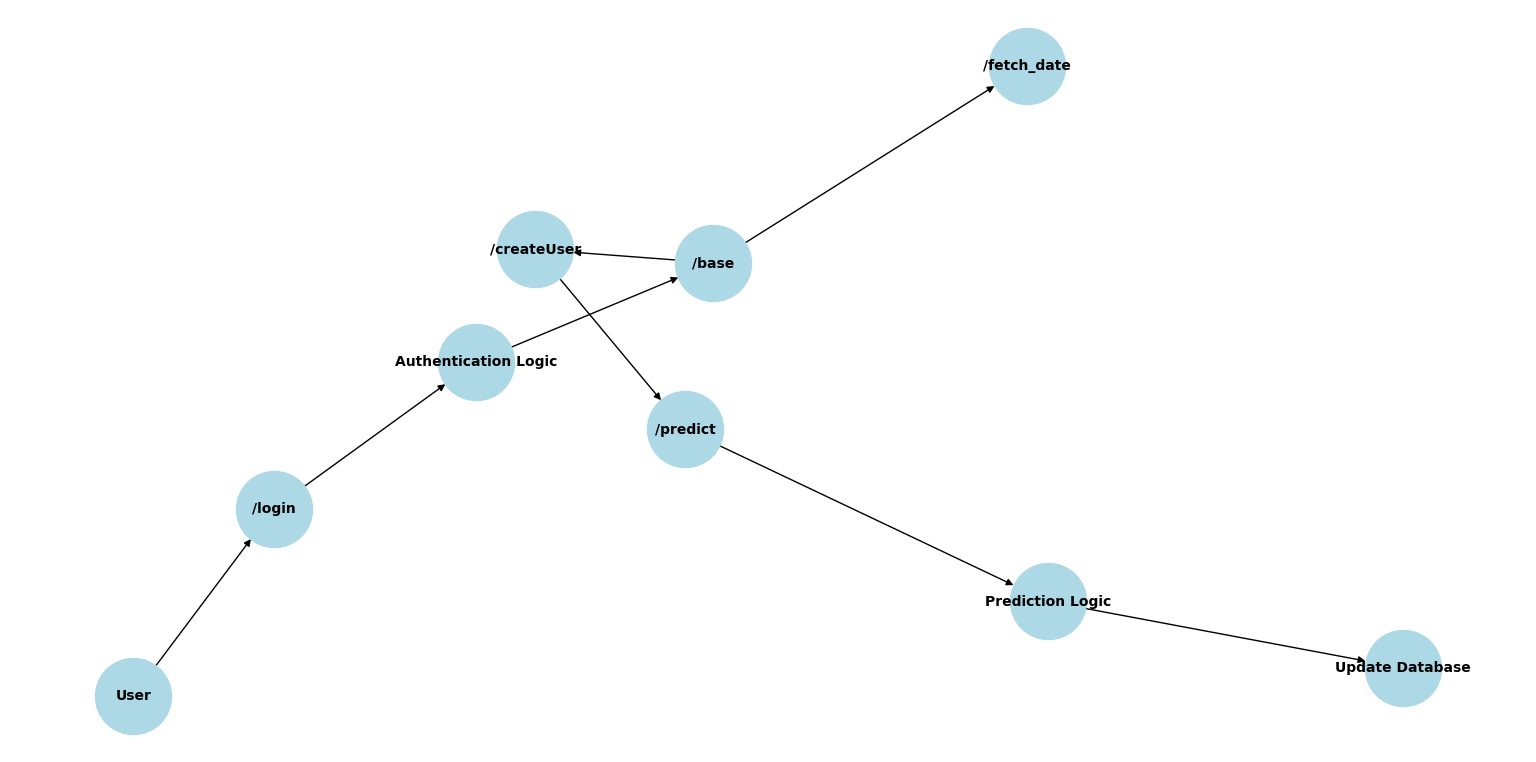
\includegraphics[width=1\linewidth]{routing_flow_diagram.png}
        \caption{Routing Flow:}
        \label{fig:enter-label}
    \end{figure}
\end{itemize}
\subsubsection{firebase.py (Database Integration)}
\begin{itemize}
    \item Purpose: This module ensures seamless interaction with Firebase Firestore, enabling real-time updates and storage of user-specific data.\newline
    \item Key Functionalities:\newline
         Storing User Data: Saves calculated goals and prediction data for each user.\newline
         Updating Nutritional Data: Dynamically updates nutritional intake information based on the user's daily consumption.\newline
         Efficient Querying: Retrieves user goals and daily progress data for visualization in the frontend.\newline
\end{itemize}
\subsubsection{calculateIndv.py (Goal Calculations)}
\begin{itemize}
    \item Purpose: Provides dynamic and personalized goal-setting for users based on their inputs and health goals. \newline
    \item Key Functionalities:\newline
       BMR Calculation: Determines the user's Basal Metabolic Rate based on age, gender, height, and weight.\newline
       TDEE Calculation: Adjusts BMR based on activity level to calculate Total Daily Energy Expenditure.\newline
       Macro Goals: Breaks down calories into carbohydrates, proteins, and fats based on the user's goal (e.g., weight loss, maintenance, or muscle gain).\newline
\end{itemize}
\subsubsection{Frontend Components (templates and static/js)}
\begin{itemize}
    \item Purpose: Provides an intuitive and visually appealing interface for users to interact with the application.\newline
    \item Key Components:\newline
         Templates:\newline
            base.html: The foundational structure for all pages, ensuring consistency in design.\newline
            modifyUser.html & createUser.html: Pages for users to input and update personal data.\newline
         Scripts:\newline
            auth.js: Handles user authentication logic.\newline
            prediction.js: Manages file previews and uploads for predictions.\newline
\end{itemize}
\newpage
\section{Use Cases}
\vspace{12pt}
\begin{figure}[h!]
    \centering
    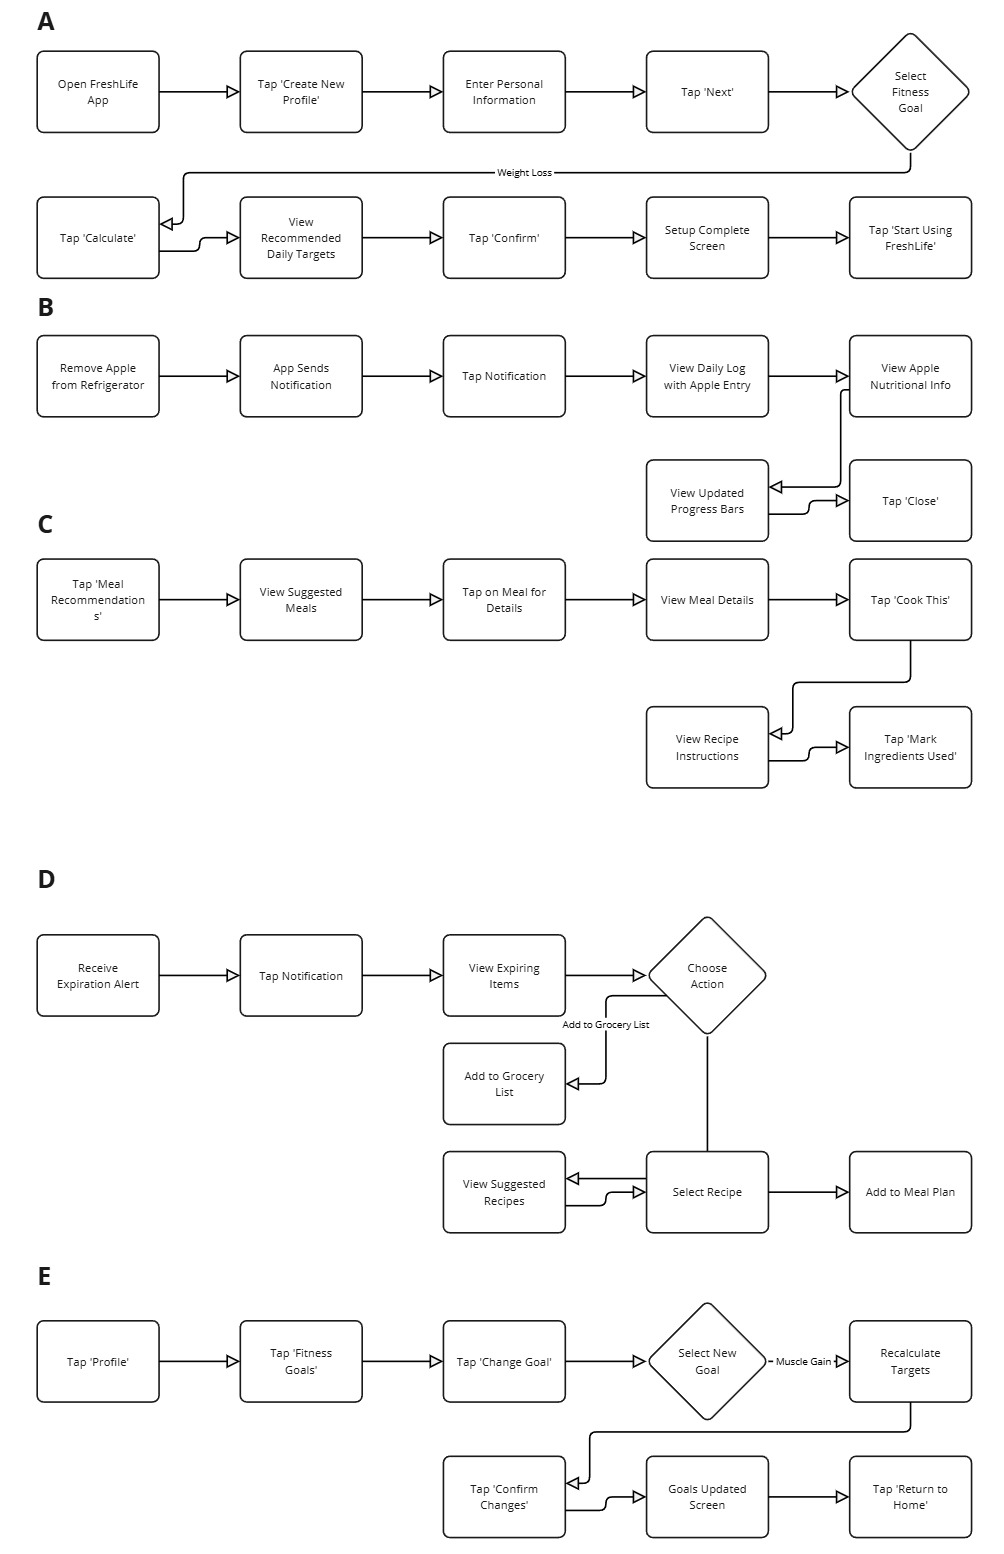
\includegraphics[scale=0.25]{Flowchart.jpg} 
    \caption{Flow Chart for Use Cases}
    \label{fig:flowchart}
\end{figure}
\subsection{Setting Up a New User Profile}
\begin{enumerate}
\item User opens the FreshLife app for the first time.
\item On the welcome screen, user taps the "Create New Profile" button.
\item In the "Personal Information" page, user enters:
\begin{itemize}
\item Age
\item Gender
\item Height
\item Weight
\item Activity level (selects from a dropdown menu)
\end{itemize}
\item User taps "Next" button.
\item On the "Fitness Goals" page, user selects their goal by tapping either:
\begin{itemize}
\item "Weight Loss"
\item "Muscle Gain"
\item "Maintain Current Weight"
\end{itemize}
\item User taps "Calculate" button.
\item App displays "Recommended Daily Targets" page showing calculated calorie and macronutrient goals.
\item User taps "Confirm" button.
\item App shows "Setup Complete" screen with a "Start Using FreshLife" button.
\item User taps this button to enter the main app interface.
\end{enumerate}
\subsection{Tracking Food Consumption}
\begin{enumerate}
\item User opens refrigerator and removes an apple.
\item FreshLife app automatically updates and sends a notification.
\item User taps the notification to open the app.
\item On the "Daily Log" page, user sees the newly added apple entry.
\item User taps on the apple entry to view detailed nutritional information.
\item At the bottom of the screen, user sees updated progress bars for daily calorie and nutrient intake.
\item User taps "Close" to return to the main "Daily Log" page.
\end{enumerate}
\subsection{Receiving Meal Recommendations}
\begin{enumerate}
\item From the app's home screen, user taps "Meal Recommendations" button.
\item On the "Meal Recommendations" page, user sees three suggested meals.
\item User taps on a meal to view details.
\item On the meal detail page, user sees ingredients, nutritional information, and a "Cook This" button.
\item User taps "Cook This" button.
\item App displays "Recipe Instructions" page with step-by-step guide.
\item At the bottom of this page, there's a "Mark Ingredients Used" button.
\item User taps this button after cooking to update the refrigerator inventory.
\end{enumerate}
\subsection{Managing Expiration Alerts}
\begin{enumerate}
\item User receives a notification about expiring milk.
\item User taps the notification to open the app to the "Expiring Items" page.
\item On this page, user sees the milk entry with two buttons: "Use in Recipe" and "Add to Grocery List".
\item User taps "Use in Recipe" button.
\item App navigates to "Suggested Recipes" page showing recipes using milk.
\item User taps on a recipe to select it.
\item On the recipe page, user taps "Add to Meal Plan" button.
\item A confirmation dialog appears, and user taps "Confirm" to add the recipe to their meal plan.
\end{enumerate}
\subsection{Adjusting Fitness Goals}
\begin{enumerate}
\item From the app's home screen, user taps "Profile" button.
\item On the "Profile" page, user taps "Fitness Goals" button.
\item On the "Fitness Goals" page, user taps "Change Goal" button.
\item A pop-up menu appears with options: "Weight Loss", "Muscle Gain", "Maintain Weight".
\item User taps "Muscle Gain" option.
\item App shows "Recalculating" screen briefly, then displays new calorie and macronutrient targets.
\item At the bottom of this page, user taps "Confirm Changes" button.
\item App shows "Goals Updated" confirmation screen with a "Return to Home" button.
\item User taps "Return to Home" to go back to the main app interface.
\end{enumerate}
\section{Discussion}
Throughout the development of the Smart Fridge System, our team faced a mix of technical challenges and non-technical hurdles. One prominent technical difficulty was integrating Firebase with our Flask backend while maintaining a robust and seamless flow of data. Specifically, managing user authentication and synchronizing nutritional data required extensive debugging and testing, especially when handling asynchronous data updates and cloud configurations.
\newline
Another technical challenge was achieving compatibility between the machine learning model for food recognition and the data retrieval mechanism. Ensuring accurate predictions while maintaining system responsiveness demanded careful preprocessing and optimization. Implementing a feature for both image and video input required updates to our frontend and backend, as well as integrating libraries like OpenCV and TensorFlow, which posed compatibility and dependency management issues.
\newline
On the non-technical side, communication among team members occasionally became difficult, especially when coordinating updates across multiple branches in GitHub. Merging changes often led to conflicts that required resolution, delaying progress. Additionally, aligning individual contributions with the overall system architecture was challenging, given the diverse skill sets and priorities within the team.
\newline
Despite these challenges, the project enhanced our problem-solving skills and deepened our understanding of collaborative software development. Looking forward, implementing a standardized workflow for team communication and documentation would mitigate these issues. Incorporating automated testing and CI/CD pipelines would also ensure better code quality and reduce integration delays.
\newline
Lastly, the experience of presenting and documenting our work has prepared us for future collaborative endeavors. The project not only showcased the importance of teamwork but also highlighted areas for personal and collective growth, particularly in version control, real-time communication, and cloud-based systems.
\newline


    

\newpage

\end{document}
